\chapter{Introduction}

\label{Introduction}

\section{Coca-cola, une emprise mondiale}

Afin de pouvoir analyser une publicité de façon efficace, j'ai décidé de directement analyser les techniques de commercialisation mises en place par la \textit{Coca-Cola Company}.
En effet, c'est en 2012 que la marque mondialement connue atteint de nouveaux sommets et devance tous ses concurrents avec des revenus de près de \textbf{48 milliards de dollars}.  Jusqu'à lors, c'était \textit{PepsiCo} qui menait le marché.
Or, le succès de Coca-Cola provient, sans aucun doute, de ces multiples réclames et campagnes publicitaires, qui, même après être passés premiers mondiaux, continuent de pulluler dans la rue, sur nos télés, nos téléphones, etc.\\
Coca-Cola n'hésite pas à investir des sommes colossales dans la réclame et la communication (avec un budget de plus de 2 milliards de dollars par an). Leurs publicités se déclinent en images fortes qui ont su s'imprimer dans la conscience collective, que ce soit avec leur ours de synthèse, avec le Père Noël ou encore par des stratégies connotés "classiques", stimulant les pulsions primaires (par exemple la soif ou la sexualité…). \parencite{Ref1}. \\


\hfill \break

\begin{figure}[th]
\centering
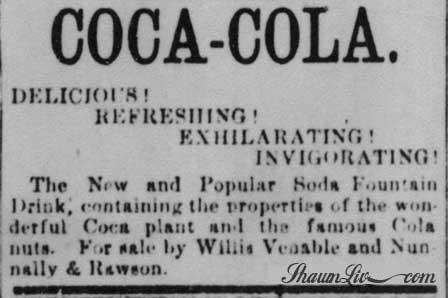
\includegraphics[width=100mm]{medias/1ere_pub}
\decoRule
\caption{1886, Atlanta - Première publicité coca-cola}
\end{figure}
\newpage

%----------------------------------------------------------------------------------------


\section{Introduction de la campagne }

Parmi les campagnes les plus célèbres que coca-cola ont publiées, j'ai choisi de me pencher sur un précurseur de la marque, une campagne qui à tellement fait parler d'elle, qu'encore aujourd'hui les gens en parlent encore et vont jusqu'à penser que le Père Noël est le fruit de la compagnie;  il s'agit de la campagne à grande échelle "\textit{coke x-mas}".
Cette campagne à vu le jour en décembre 1930, à cette période-là, coca-cola était une boisson gazeuse locale aux Américains, exclusivement réservée aux périodes estivales.
Voulant "rafraîchir" et étendre la marque, cette campagne eue alors deux objectifs : 

\begin{itemize}
\item Trouver un moyen, avec une image ou un symbole mondialement connu, de s'exporter ;
\item Couvrir plus de saisons, afin d'augmenter les ventes;
\end{itemize}

\begin{figure}[th]
\centering
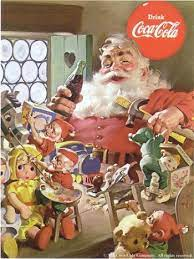
\includegraphics[width=70mm]{medias/perenoel1}
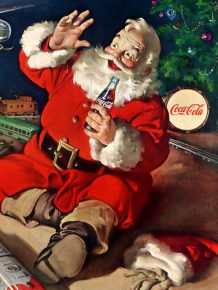
\includegraphics[width=70mm]{medias/perenoel2}
\decoRule
\caption{1935/1361 - Quelques réclames de la campagne "coke x-mas"}
\end{figure}
